% !TEX root = ../../main.tex
% !TeX spellcheck = de_DE

\chapter{Ergebnisse}

\section{Dense-GAN}
Über das Tensorboard können die generierten Daten in verschiedenen Ansichten angezeigt werden.
Die wichtigste ist die Hyperparameter-Ansicht.
Wie in Abbildung \ref{ergebnis:densegan-hyper} zu erkennen ist, werden nicht nur alle Parameterkombinationen angezeigt.
Es wird auch dargestellt, zu welchen Metriken diese Kombinationen geführt haben.
Damit lässt sich leicht evaluieren, welche Hyperparameter die besten Ergebnisse erzeugt haben.

\begin{figure}[H]
	\centering
	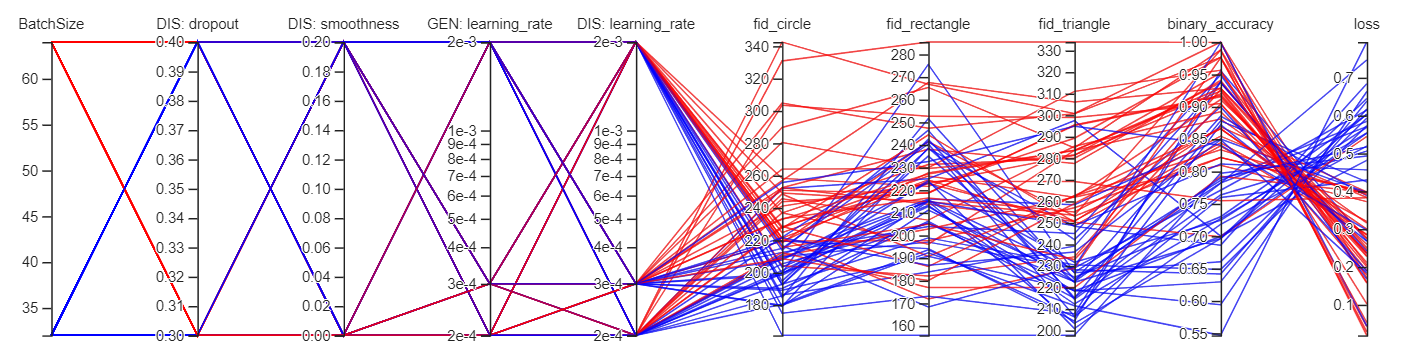
\includegraphics[width=0.75\textheight]{kapitel/5_ergebnisse/densegan/hyperparameter.PNG}
	\caption{Hyperparameter-Ansicht des Dense-GAN}
	\label{ergebnis:densegan-hyper}
\end{figure}

Auf der linken Seite sind alle Hyperparameter aufgelistet.
Die Abkürzung \textit{GEN} steht dabei für den Generator und \textit{DIS} repräsentiert den Diskriminator.
Außerdem können die einzelnen Graphen in einem Farbverlauf von Rot nach Blau einsortiert werden.
Dadurch kann der Einfluss von einzelnen Hyperparametern deutlich visualisiert werden.
\newline

In der Abbildung \ref{ergebnis:densegan-hyper} wurde nach der BatchSize sortiert.
Es ist deutlich zu erkennen, dass ein Wert von 32 (hier blau) bessere FID-Werte als 64 (hier rot) erzielt.
Im Gegensatz dazu steht die Smoothness und der Dropout.
Bei den gewählten Werten lassen sich kaum Tendenzen erkennen, wie in der Abbildung \ref{ergebnis:densegan-hyper-smoot-drop} visualisiert ist.

\begin{figure}[H]
	\centering
	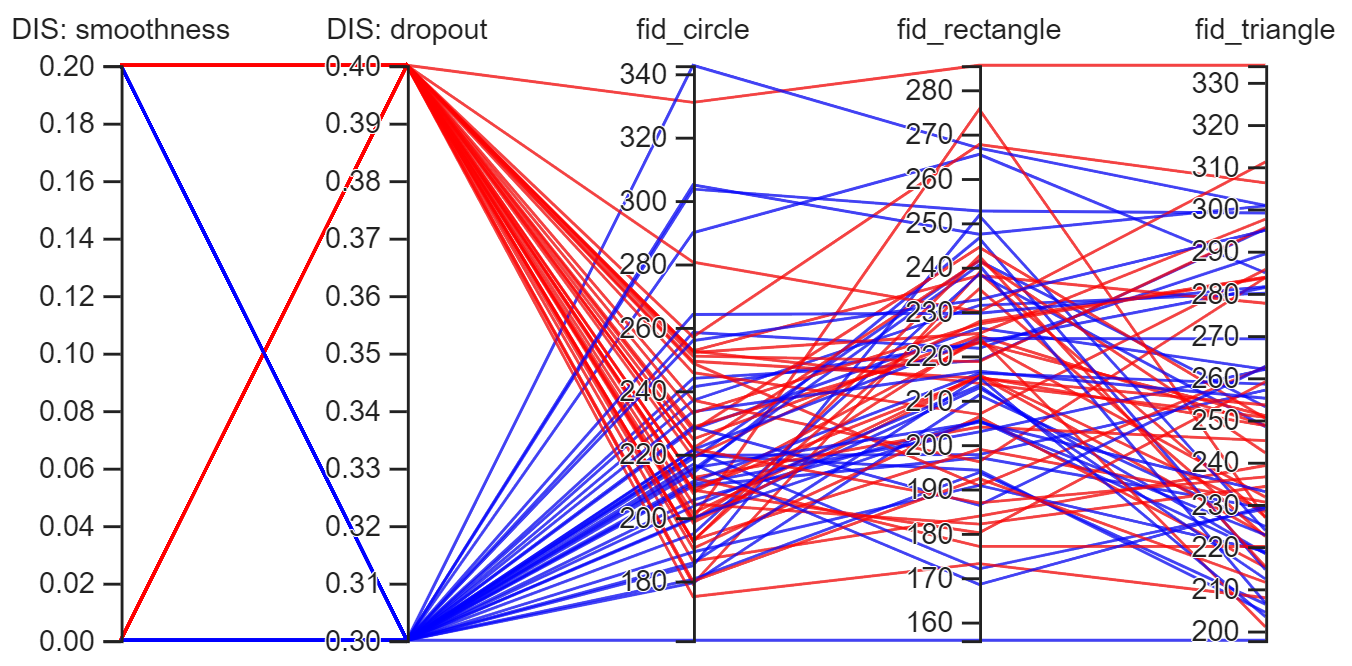
\includegraphics[width=0.6\textheight]{kapitel/5_ergebnisse/densegan/hyperparameter_dropout_smooth.PNG}
	\caption{Einfluss von Smoothness und Dropout auf das Dense-GAN}
	\label{ergebnis:densegan-hyper-smoot-drop}
\end{figure}

Bei der Lernrate wurden die besten Ergebnisse bei gleichen Werten für Diskriminator und Generator erreicht.  
In der Abbildung \ref{ergebnis:densegan-lr} ist zu erkennen, dass bei einer Lernrate von \(2e-3\) (a), die niedrigsten FID-Werte erreicht wurden.
Ähnlich niedrige Werte wurden mit Lernraten zwischen \(2e-4\) und \(3e-4\) erreicht, wie im rechten Teil (b) zu erkennen ist.
 
 \begin{figure}[H]
 	\centering
 	\subfloat[][]{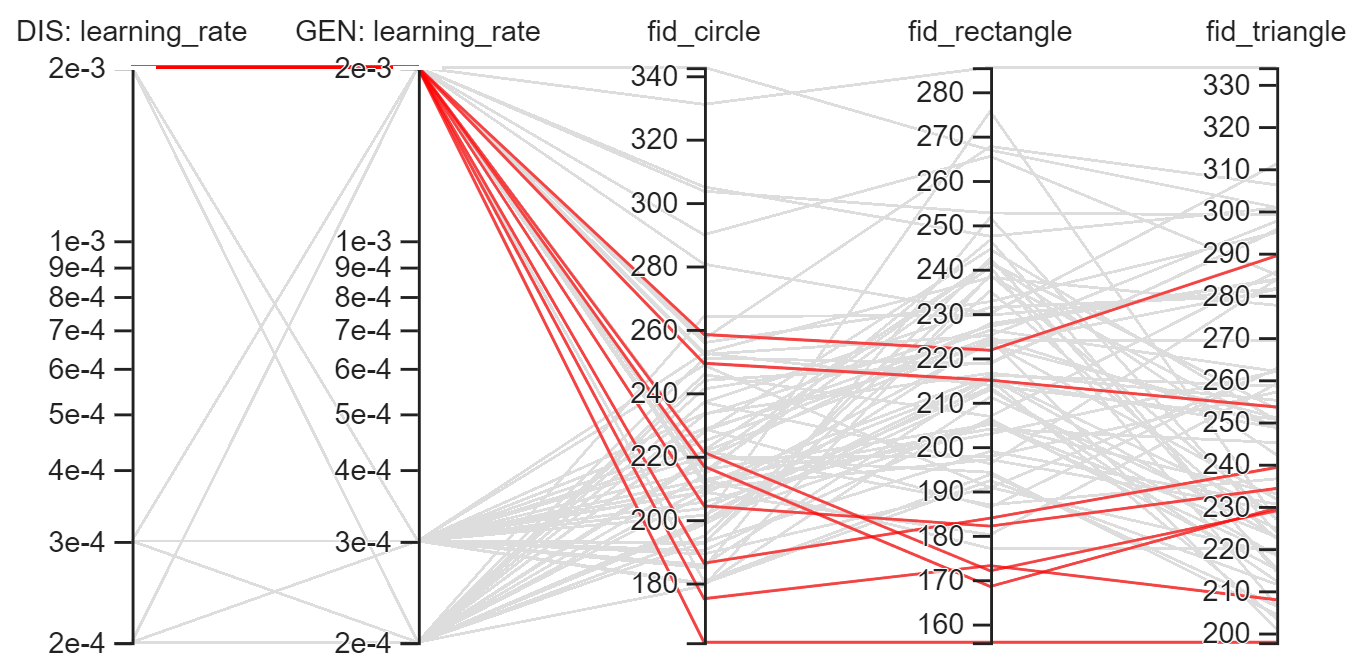
\includegraphics[width=0.45\linewidth]{kapitel/5_ergebnisse/densegan/hyperparameter_lr_same.PNG}}
 	\qquad
 	\subfloat[][]{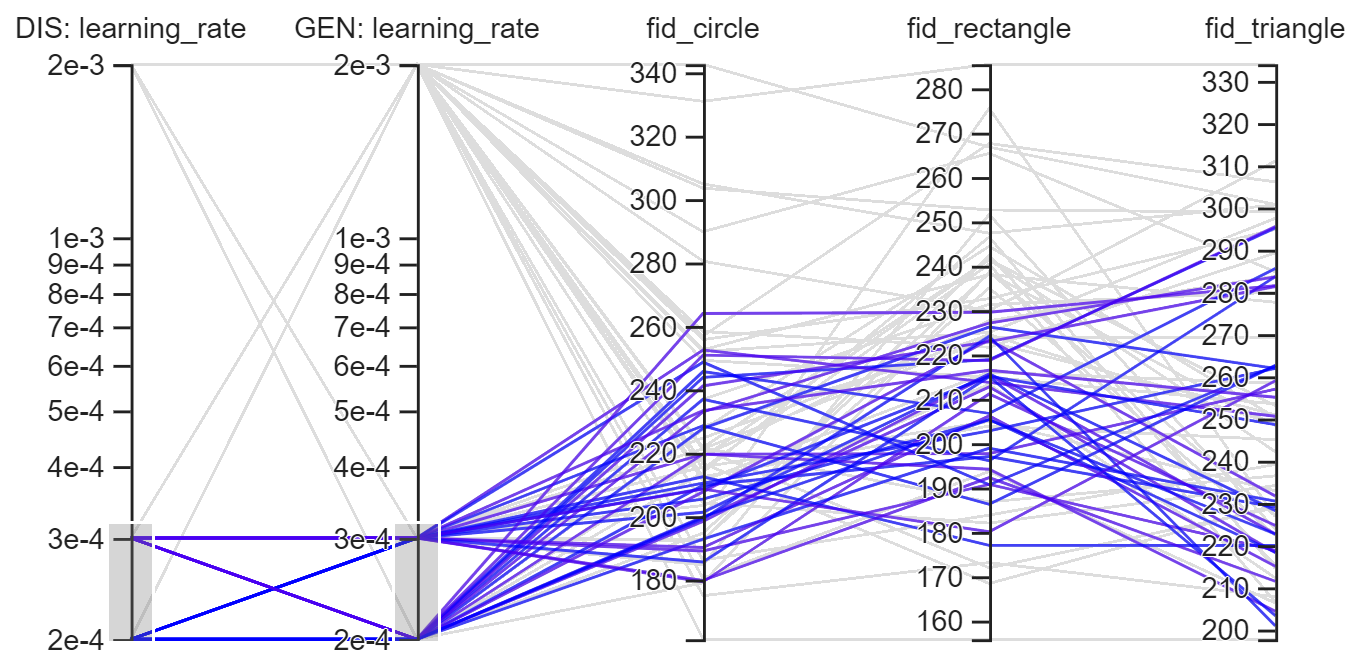
\includegraphics[width=0.45\linewidth]{kapitel/5_ergebnisse/densegan/hyperparameter_lr_low.PNG}}
 	\caption{Einfluss der Lernrate auf die FID-Werte des DENSE-GAN}
 	\label{ergebnis:densegan-lr}
 \end{figure}

\subsection{Bilder}
Wie bereits beschrieben, werden neben den Hyperparameter und Metriken auch generierte Bilddaten protokolliert.
Neben den FID-Werten, kann so die generierten Ergebnisse subjektiv Bewerter werden.
Die subjektiv besten Figuren sind in der Abbildung \ref{ergebnis:densegan-best} (a) zu sehen.
Die Figuren mit den besten FID-Werten werden in der Abbildung  \ref{ergebnis:densegan-best} (b) gezeigt.
Es lässt sich leicht erkennen, das die subjektive Bewertung und FID-Werte nicht übereinstimmen.

\begin{figure}[H]
	\centering
	\subfloat[][]{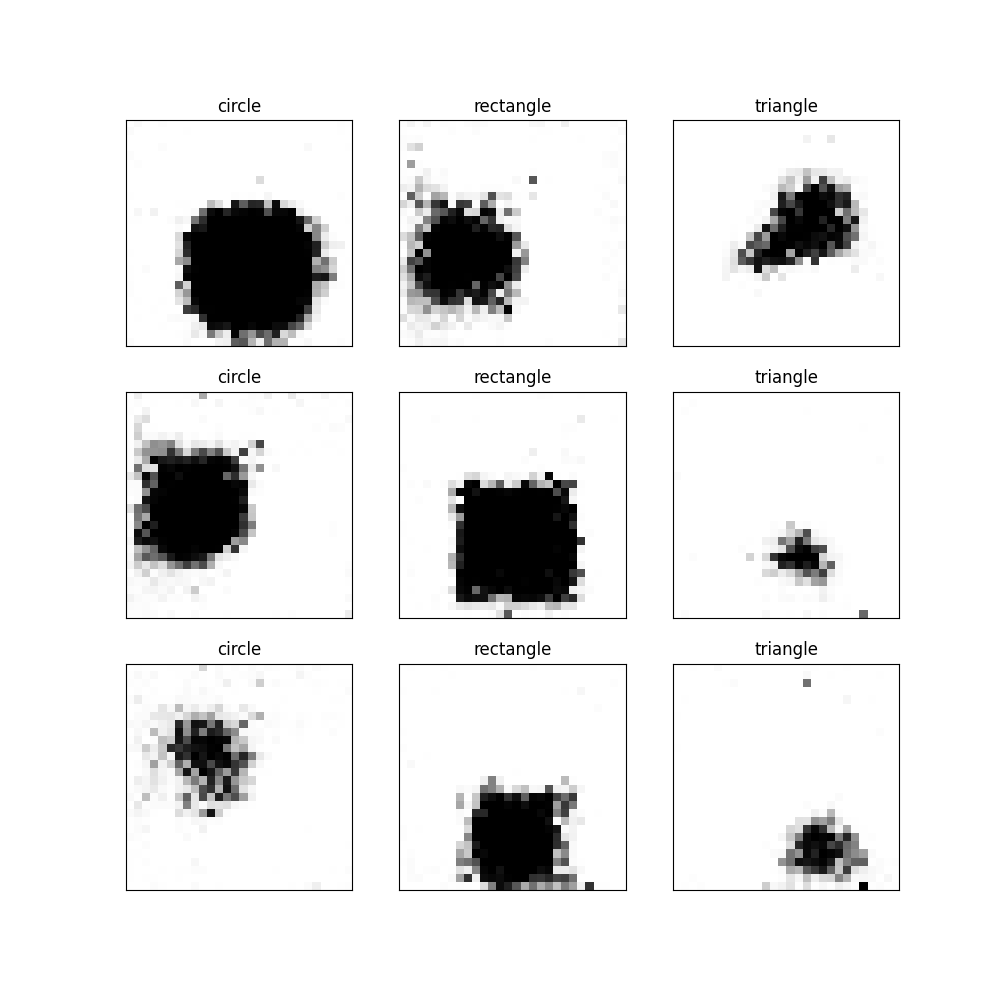
\includegraphics[width=0.45\linewidth]{kapitel/5_ergebnisse/densegan/good_example.png}}
	\qquad
	\subfloat[][]{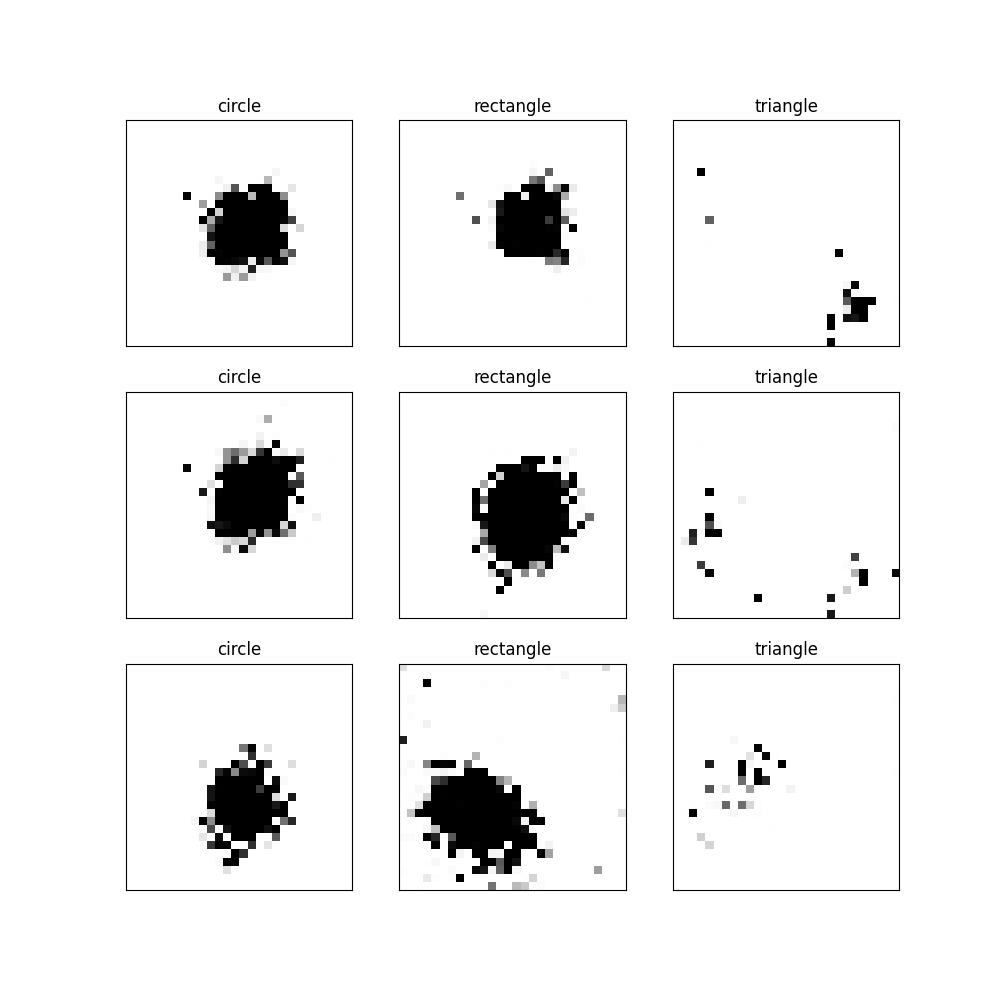
\includegraphics[width=0.45\linewidth]{kapitel/5_ergebnisse/densegan/best_fid.png}}
	\caption{Beste Ergebnisse bemessen nach subjektiver Bewertung und FID-Werte}
	\label{ergebnis:densegan-best}
\end{figure}

Da das erste Beispiel gute Ergebnisse erzeugt, wurde ein GAN mit den gleichen Hyperparametern für 1000 Epochen trainiert.
Auch wenn eine große Menge an Bildartefakte zu erkennen ist, stechen die Kanten der Formen deutlicher heraus (siehe Abbildung \ref{ergebnis:densegan-good-example-long}).

\begin{figure}[H]
	\centering
	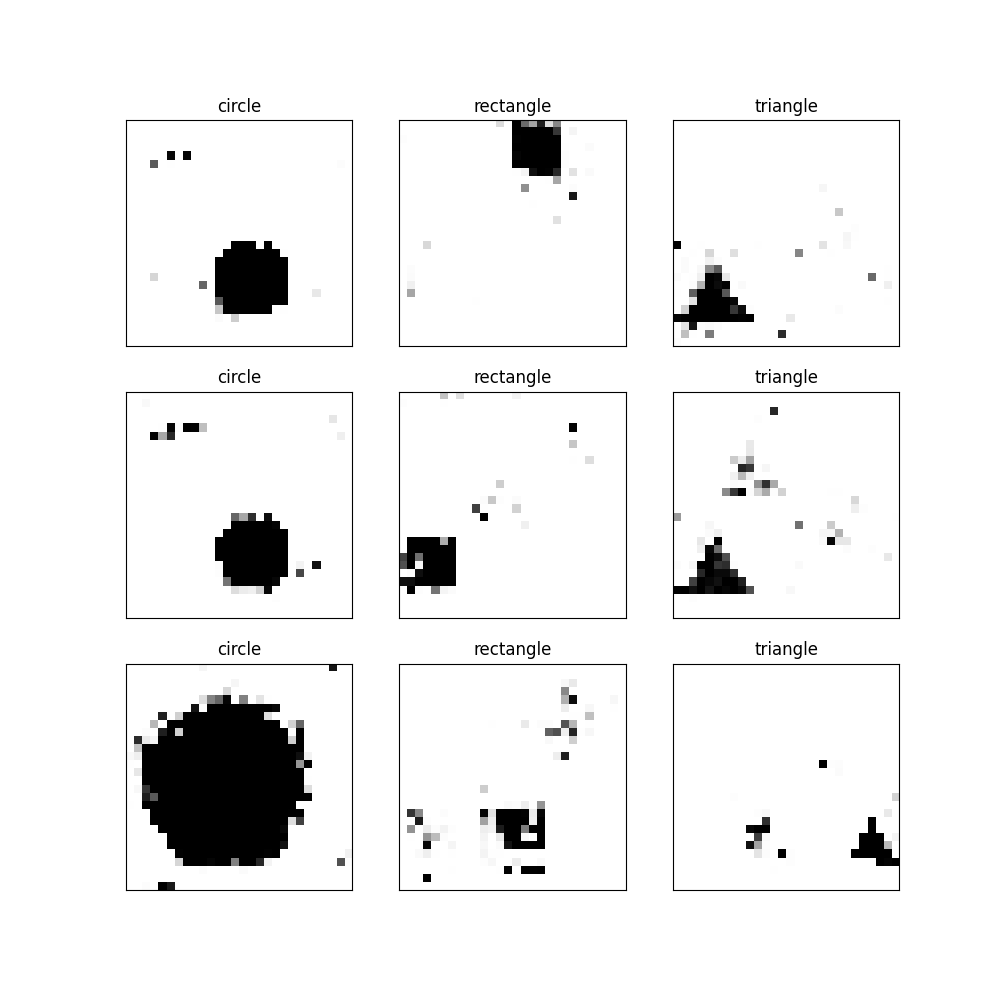
\includegraphics[height=0.4\textheight]{kapitel/5_ergebnisse/densegan/good_example_long.png}
	\caption{Ergebnis von 1000 Epochen Training}
	\label{ergebnis:densegan-good-example-long}
\end{figure}

\section{DC-GAN}
Im Vergleich zum Dense-GAN, sind wie in Abbildung \ref{ergebnis:dcgan-hyper} zu sehen, weniger Hyperparameter Kombinationen getestet worden.
Dadurch ist das Tensorboard weniger dicht befüllt und deutlich übersichtlicher.

\begin{figure}[H]
	\centering
	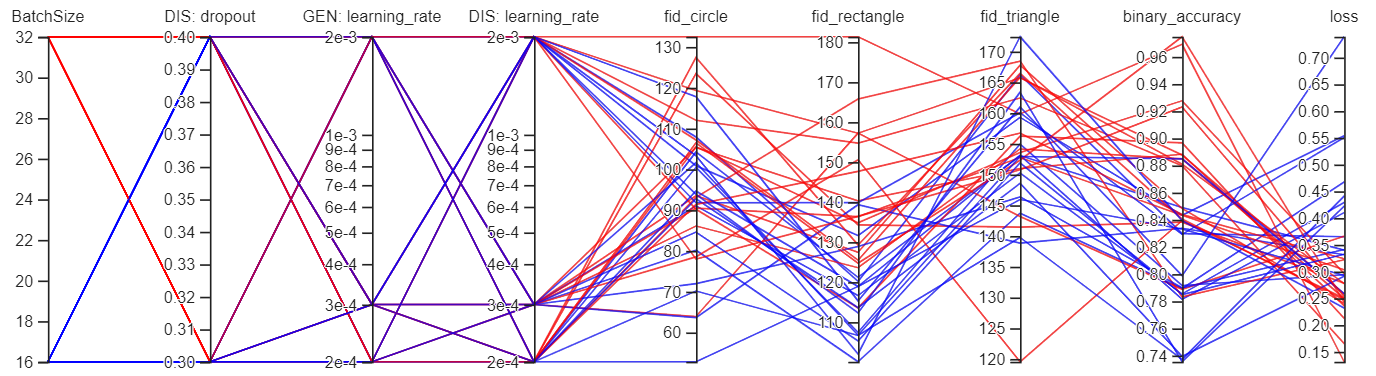
\includegraphics[width=0.75\textheight]{kapitel/5_ergebnisse/dcgan/hyperparameter.PNG}
	\caption{Hyperparameter-Ansicht des DC-GAN}
	\label{ergebnis:dcgan-hyper}
\end{figure}

Die kleinere BatchSize von 16 wirkt sich postive auf die FID-Werte des Kreis und Quadrats aus.
Nur beim FID-Wert der Dreiecke gibt es einen deutlichen Ausreißer, welcher eine BatchSize von 32 bevorzugt.
\newline

Die Smoothness fällt bei dieser Hyperparametersuche heraus.
Der Dropout jedoch, hat nur einen kleinen Einfluss auf das Ergebnis. 
Das kann in Abbildung \ref{ergebnis:dcgan-hyper-dropout} betrachtet werden.

\begin{figure}[H]
	\centering
	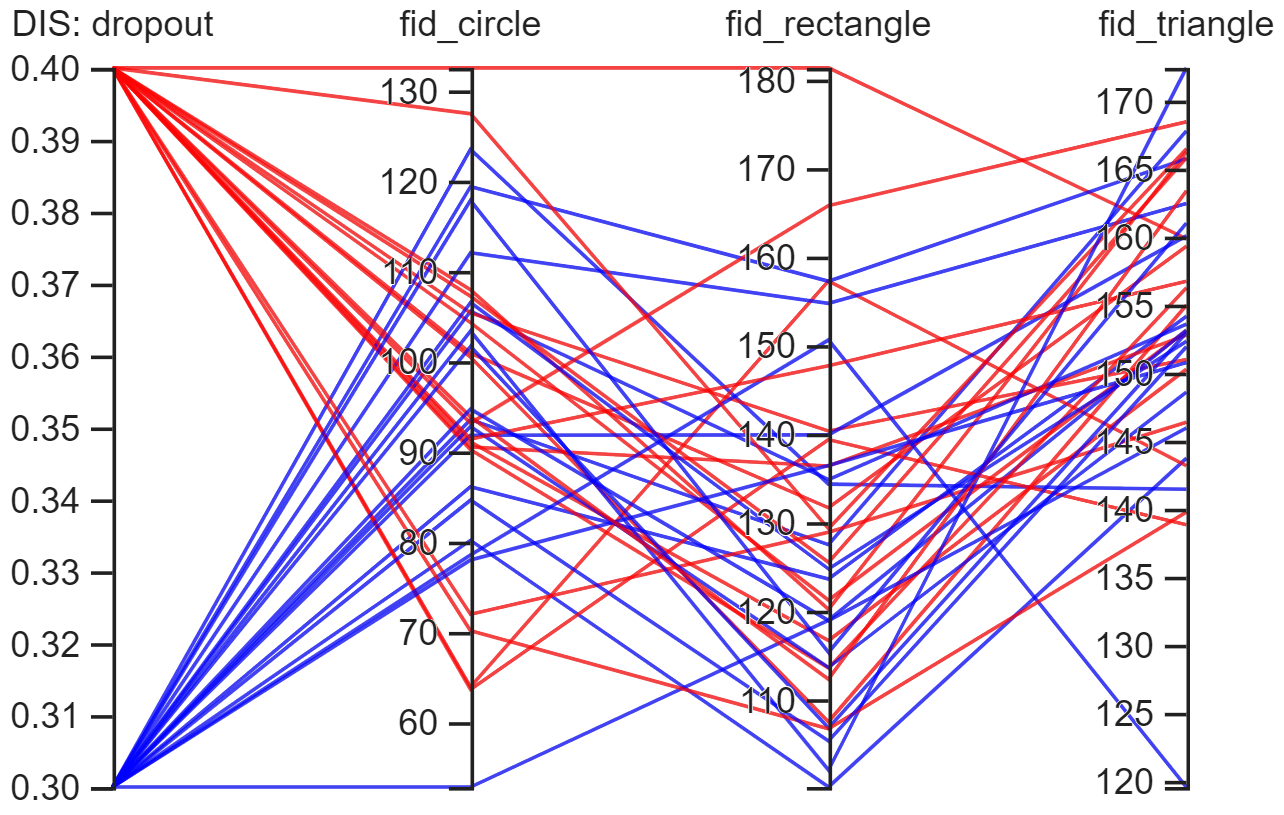
\includegraphics[width=0.5\textheight]{kapitel/5_ergebnisse/dcgan/hyperparameter_droupout.PNG}
	\caption{Einfluss des Droupouts auf das DC-GAN}
	\label{ergebnis:dcgan-hyper-dropout}
\end{figure}

Bei einer beidseitigen Lernrate von \(2e-3\), sind zwar die FID-Werte der Quadrate tendenziell klein, jedoch gilt das nicht für die anderen beiden Figuren.
Dies kann man gut in der Abbildung \ref{ergebnis:dcgan-lr} (a) erkennen.
Im Gegenzug ist bei einer deutlich kleineren Diskriminator-Lernrate im Bereich von \(2e-4\) bis \(3e-4\) und gleichbleibenden Generator-Lernrate von \(2e-3\), das Ergebnis umgekehrt.
In der Abbildung \ref{ergebnis:densegan-lr} (b) wird visualisiert, dass die FID-Werte der Kreise und Dreiecke minimal werden.
Zwar nimmt die Metrik für das Quadrat nicht den kleinsten Wert an, jedoch bewegen sich die Ergebnisse auch hier im niedrigen Bereich. 

\begin{figure}[H]
	\centering
	\subfloat[][]{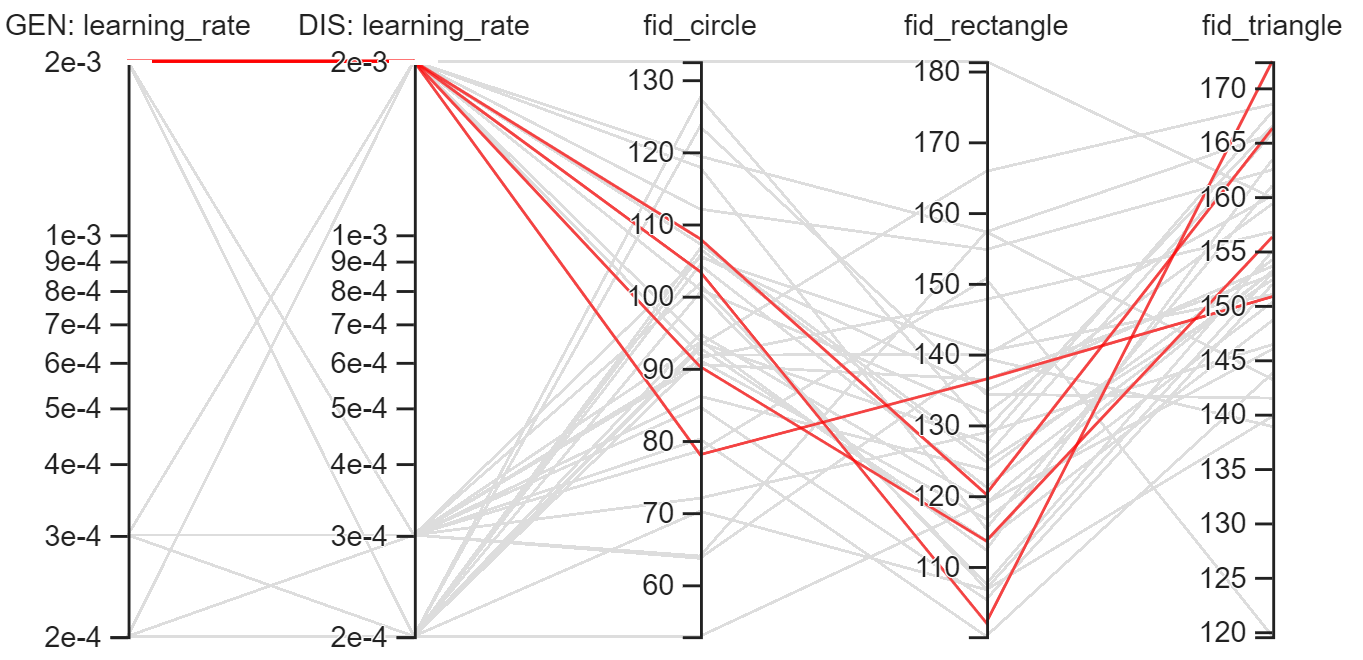
\includegraphics[width=0.45\linewidth]{kapitel/5_ergebnisse/dcgan/hyperparameter_lr_same.PNG}}
	\qquad
	\subfloat[][]{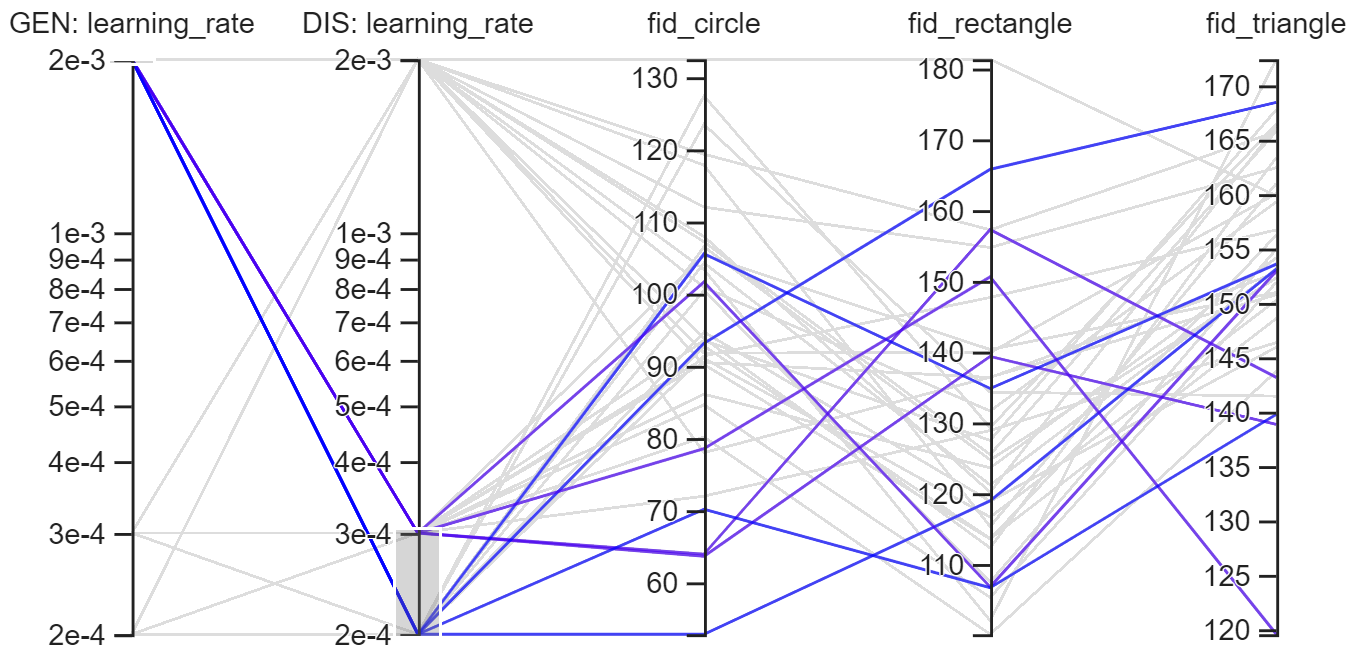
\includegraphics[width=0.45\linewidth]{kapitel/5_ergebnisse/dcgan/hyperparameter_lr_not_same.PNG}}
	\caption{Einfluss der Lernrate auf die FID-Werte des DC-GAN}
	\label{ergebnis:dcgan-lr}
\end{figure}

\subsection{Bilder}
Die niedrigsten FID-Werte wurden jeweils bei anderen Hyperparameter-Kombinationen erreicht.
Sie können in der Abbildung \ref{ergebnis:dcgan-fid} betrachtet werden, wobei die besten Kreise in (a), Quadrate in (b) und Dreiecke in (c) zu sehen sind.
In der subjektiven Suche konnte kein Training gefunden werden, welches eine Generierung von glaubhaften Bildern ermöglicht.


\begin{figure}[H]
	\centering
	\subfloat[][]{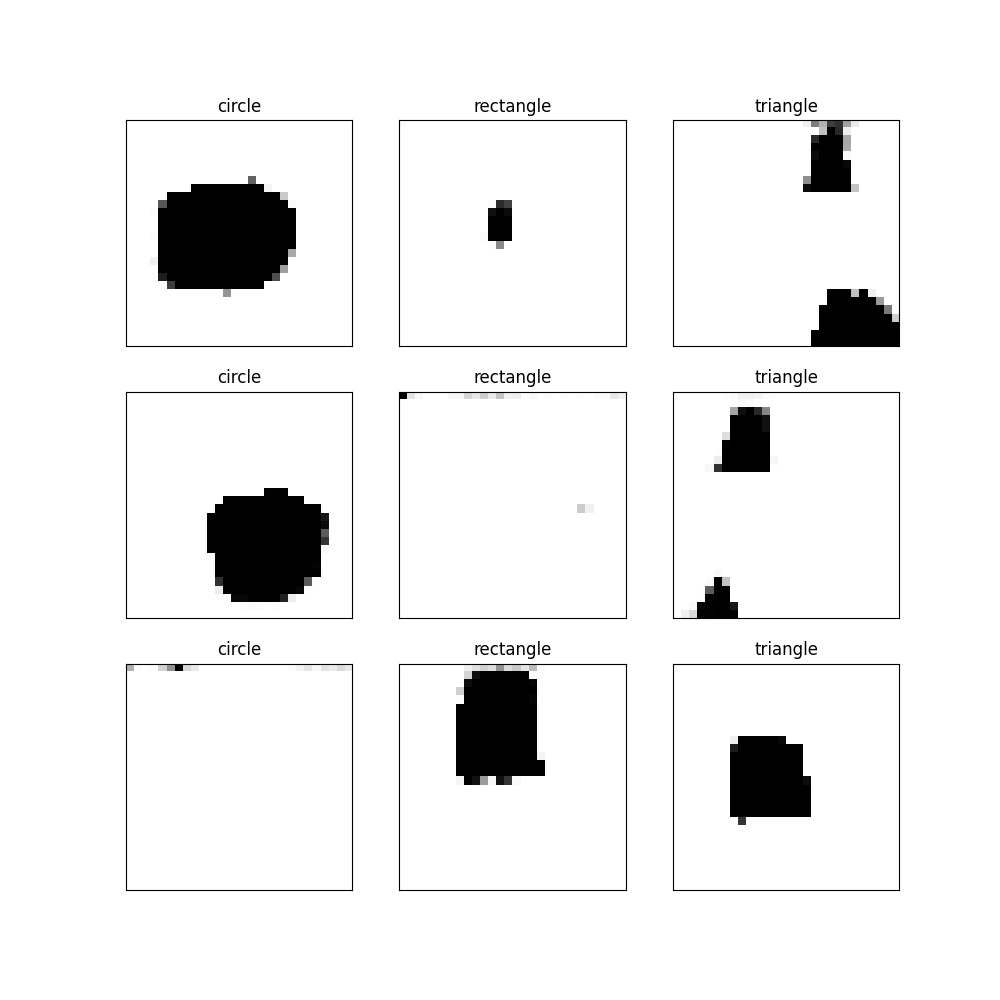
\includegraphics[width=0.45\linewidth]{kapitel/5_ergebnisse/dcgan/fid_circle.png}}
	\qquad
	\subfloat[][]{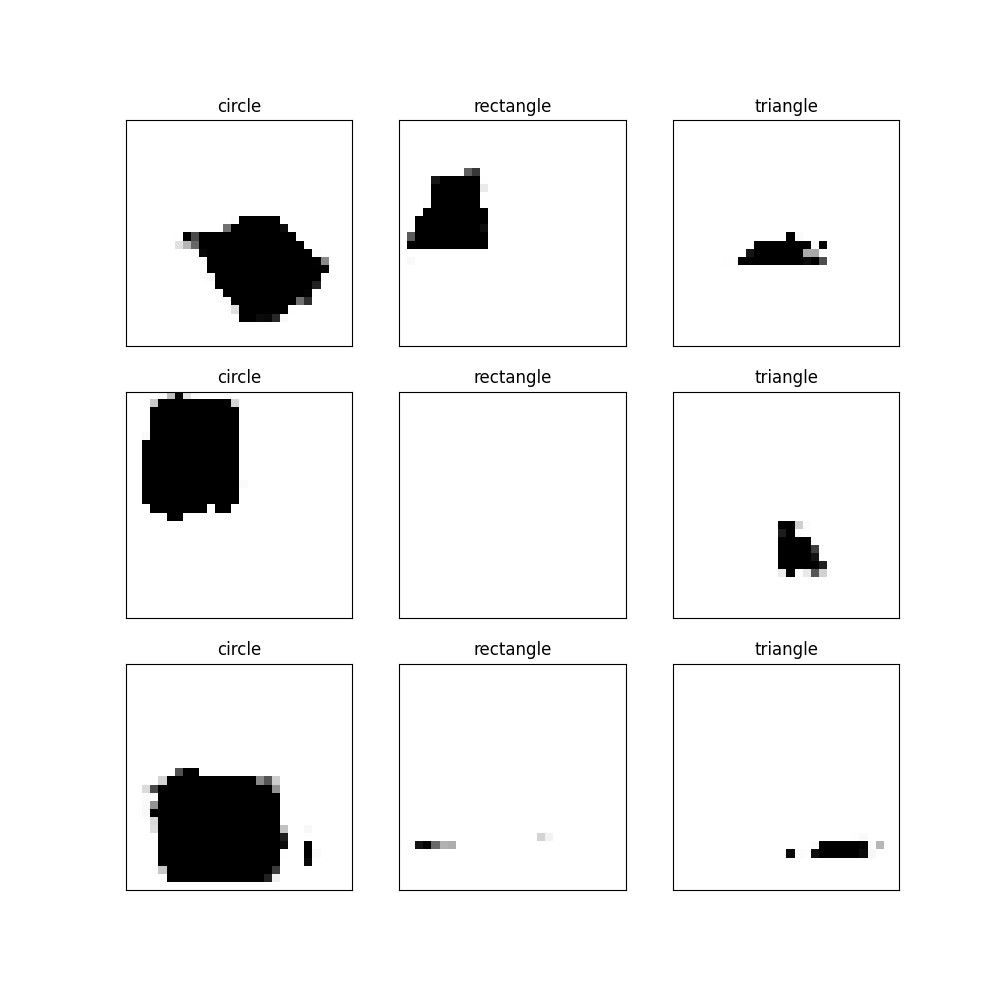
\includegraphics[width=0.45\linewidth]{kapitel/5_ergebnisse/dcgan/fid_rec.png}}
	\qquad
	\subfloat[][]{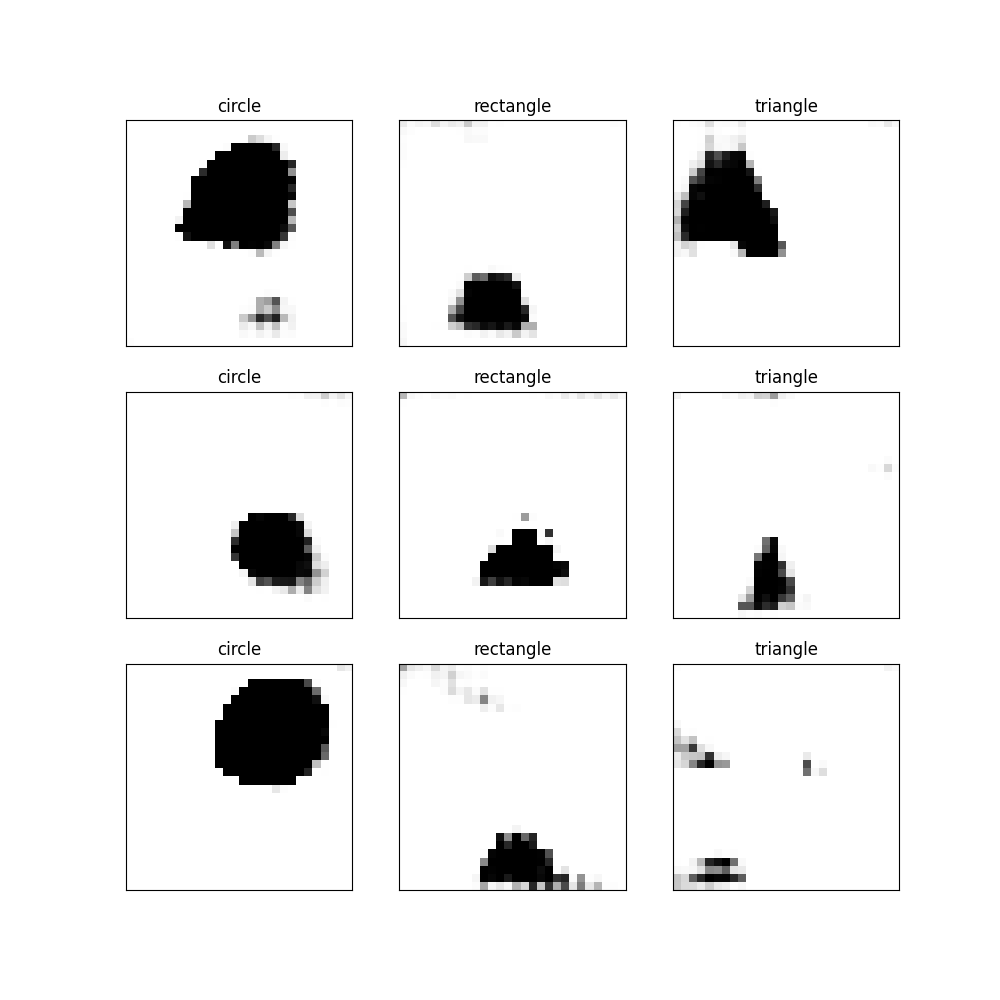
\includegraphics[width=0.45\linewidth]{kapitel/5_ergebnisse/dcgan/fid_tri.png}}
	\caption{Niedrigsten FID-Werte beim DC-GAN}
	\label{ergebnis:dcgan-fid}
\end{figure}

\section{DC Generator und Dense Discriminator}

\section{Dense Generator und DC Discriminator}

\section{DC-GAN-Medical-Inspired}
\begin{itemize}
	\item Tensorboard grafik
	\item Beste Bilder
	\item Hyperparameter Analyse
\end{itemize}
